\documentclass[listof=totocnumbered,bibliography=totocnumbered,12pt,oneside]{scrreprt}
\def\@afterindentfalse{\let\if@afterindent\iffalse}
\usepackage[english,german,ngerman]{babel}
\usepackage{xltxtra}
\usepackage{lmodern}
\usepackage{textcomp}
\usepackage{graphicx}
\usepackage{chngcntr}
\usepackage{amsmath,amsfonts}
\usepackage{fancyvrb}
\usepackage{minted}
\usepackage{color}
\usepackage{url}
\usepackage{setspace}
\usepackage[noindentafter]{titlesec}
\usepackage{titletoc}
\usepackage{fancyhdr}
\usepackage{lastpage}

\newfontfamily\headingfont[]{Avenir Heavy}
\definecolor{codebg}{rgb}{0.8,0.8,0.9}
\newminted{c++}{linenos=true,bgcolor=codebg,tabsize=4,showspaces=false}
\setcounter{secnumdepth}{3}
\setcounter{tocdepth}{3}
\counterwithout{footnote}{chapter}
\numberwithin{equation}{subsection}
\renewcommand\theequation{\arabic{equation}}
\setmainfont[Mapping=tex-text]{Avenir Book}
\setsansfont{Avenir Book}
\titleformat{\tableofcontents}{\Large\bfseries}{\headingfont}{0em}{}
\titleformat{\chapter}{\Large\bfseries}{\headingfont}{0em}{\thechapter\hspace{1em}}
\titleformat{\section}{\large\mdseries}{\headingfont}{0em}{\thesection\hspace{1em}}
\titlespacing{\paragraph}{0pt}{3.5ex plus 1ex minus .2ex}{0pt}
\linespread{1.3}

\lhead[O,E]{}
\rhead[O,E]{Door Tracked AR}
\lfoot[O,E]{Seite \thepage\ von \pageref{LastPage}}
\cfoot[O,E]{}
\rfoot[O,E]{Kron, Ilic}
\renewcommand{\headrulewidth}{0.4pt}
\renewcommand{\footrulewidth}{0.4pt}

\fancypagestyle{plain}{
	\lhead[O,E]{}
	\rhead[O,E]{Door Tracked AR}
	\cfoot[O,E]{}
	\rfoot[O,E]{Kron, Ilic}
}

\begin{document}
\pagestyle{fancy}

\subject{Bachelor-Thesis}
\title{Door Tracked Augmented Reality}
\author{Mato Ilic \and David Kron}
\date{Januar 2014}
\publishers{Betreuer: Marcus Hudritsch\\Experte: Andreas Dürsteler}

\maketitle

\chapter{Abstract}
Thema dieser Arbeit war, eine Augmented Reality Anwendung zu erstellen, welche Türen erkennt und Objekte (z.B. ein Vordach) über dieser Projeziert. Die Projektion soll dabei perspektivisch korrekt sein. Sprich, steht der Anwender seitlich zur Tür, dann sieh er auch das Vordach von der Seite. Die Anwendung sollte möglichst Plattformunabhängig sein. Aus diesem Grund sollten möglichst alle verwendeten Bibliotheken Teil des Projektes sein und spezifisch für dieses kompiliert werden. So soll die Installation erleichtert werden. Zur Umsetzung wurde die OpenCV Bibliothek verwendet, welche eine plattformübergreifendes Toolset für die Bildverarbeitung bietet. Die Darstellung der Ausgabe geschieht mittels OpenGL.
\newpage

\tableofcontents
\newpage

\chapter{Einleitung}

Augmented Reality oder kurz AR ist eine computergestützte Erweiterung der Realitätswahrnehmung. Im Vergleich zur Virtual Reality, wo der Anwender in eine komplett künstlich generierte Welt eintaucht, geht es bei AR primär darum zusätzliche Informationen anzuzeigen, welche sich bestmöglich in die Umgebung einpassen. AR kann alle menschlichen Sinne erweitern, jedoch beschränkt sich die heutige Technologie primär darauf Live-Bilder oder Videos mit Zusatzinformationen mittels Einblendung oder Überlagerung zu ergänzen.

\section{Anwendungsgebiete}

Augmented Reality kann in allen Bereichen des Alltags eingesetzt werden. Bei der Navigation im Auto oder im Gebäude können Routen und Hinweise direkt in die Umgebung integriert werden, so dass der Benutzer nie das Auge von der Strasse abwenden muss. Ärzten kann AR dabei helfen gezielter zu arbeiten indem Röntgenaufnahmen während der Operation direkt auf den Patienten projiziert werden. Die Grundlagen hierfür sind meist die Gleichen wie in diesem Projekt. Objekterkennung, Positionsbestimmung und die Integration der Zusatzinformationen in die Umgebung.

\subsection{Medizin}

\begin{figure}[!ht]
\centering
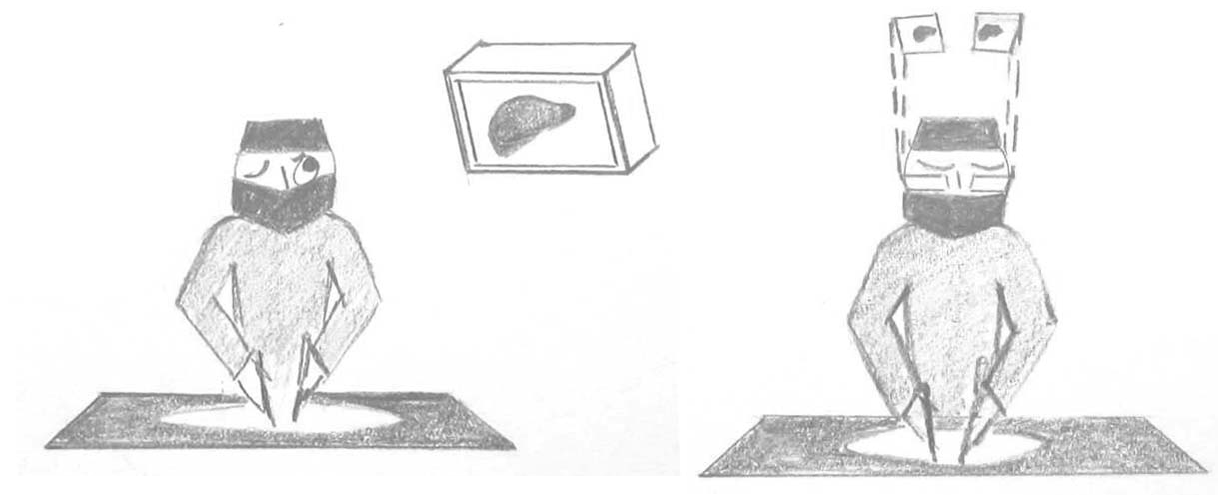
\includegraphics[scale=0.3]{images/vorteile_augmented_reality_medizin} 
\caption{Quelle: Suthau Tim, Berlin 2006, entnommen aus: Positionsgenaue Einblendung räumlicher Informationen in einem See Through Head Mounted Display für die Medizin am Beispiel der Leberchirurgie [Seite 13]}
\label{fig:ar-medicine}
\end{figure}

In der Medizin sind die Anwendungsmöglichkeiten von Augmented Reality vielfältig. Von der OP-Planung über die visuelle Navigation während der OP bis hin zur Telemedizin. Unterlagen wie Checklisten können zur Planung direkt Objektbezogen eingeblendet werden. So kann immer verfolgt werden wie die Vorbereitung des Patienten voranschreitet. Bei der Einrichtung des Operationssaals kann mittels AR direkt angezeigt werden, wo alles stehen muss um einen reibungslosen Ablauf der Operation zu garantieren. Während der Operation kann sich der Arzt voll und ganz auf den Patienten konzentrieren. Anstatt dass er seinen Blick immer wieder abwenden muss um z.B. Röntgenaufnahmen zu betrachten, werden diese direkt in das Sichtfeld projiziert. Speziell bei minimalinvasiven Eingriffen können so auch direkt die Navigationswege dargestellt werden, was die Präzision des Eingriffes erhöht.
\paragraph{}
Im Bereich der Telemedizin können Spezialisten dem ausführenden Arzt Hilfestellungen während der Diagnose oder Operation einblenden. Mediziner können so weltweit in Echtzeit kooperieren.

\subsection{Marketing}

\begin{figure}[!ht]
\centering
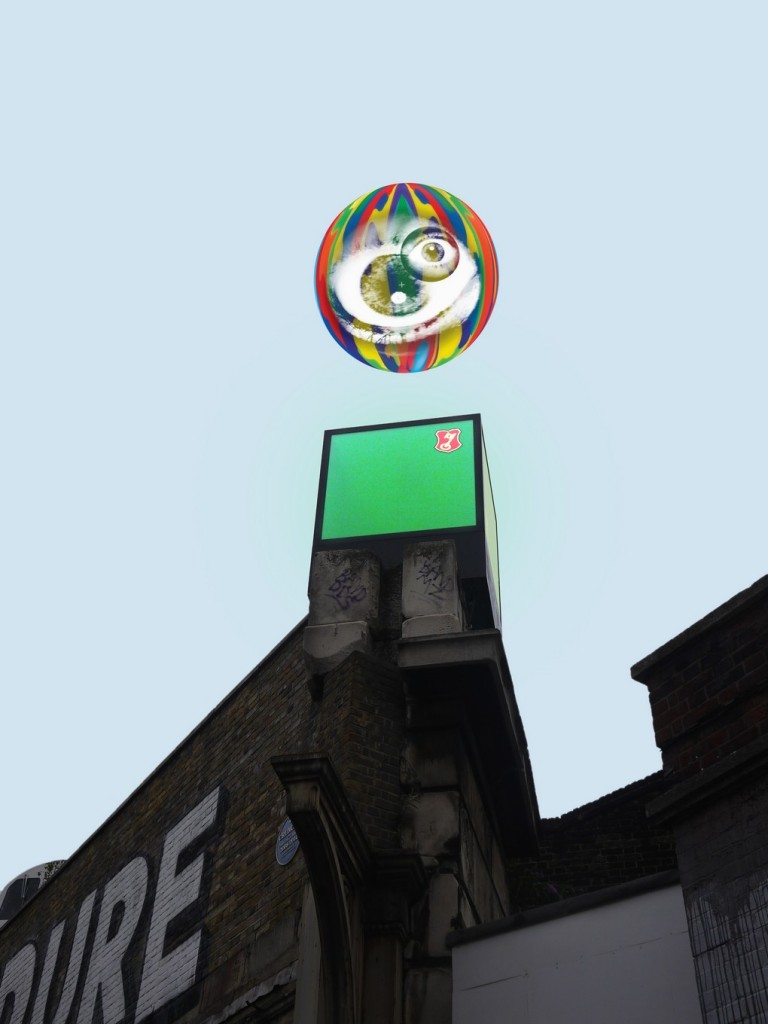
\includegraphics[scale=0.3]{images/ar-marketing} 
\caption{Becks Green Box Kampagne. Quelle: http://www.i-ref.de/2011/12/06/beck's-green-box-projekt-augmented-reality-in-berlin}
\label{fig:ar-marketing}
\end{figure}

Auch im Bereich des Marketing bietet Augented Reality unzählige neue Möglichkeiten. Tablets und Smartphones sind fester Bestandteil des Alltags geworden. Bietet man den Kunden die Möglichkeit Produkte und Brands interaktiv in ihrer Umgebung zu entdecken, so hinterlässt dies einen bleibenden Eindruck und erhöht die Bindung zur Marke. Ein Vorreiter war hier die Firma Becks im vergangenen Jahr. Um den Kunden das Produkt näher zu bringen hat Becks in Grossstädten weltweit grüne Boxen aufgestellt. Haben die Benutzer ihr Smartphone dann auf diese gerichtet, bot sich ihnen eine bunte 3D-Show. Direkt in ihrer gewohnten Umgebung im Herzen der Städte. Nach dieser Kampagne konnte Becks einen signifikaten Anstieg des Absatzes in der betroffenen Städten feststellen und gewann weltweit neue Fans.

\paragraph{}
Dies sind nur zwei mögliche Anwendungsgebiete. Bereits wird AR auch in der Automobilbranche in Form von Overhead Displays eingesetzt. Im Militärbereich wird AR für die Einsatzkoordination in Kriegsgebieten verwendet.

\section{Aktuelle Entwicklungen}

\begin{figure}[!ht]
\centering

\includegraphics[width=\textwidth]{images/google-glass} 
\caption{Google Glass. Quelle: http://www.google.com/glass/start}
\label{fig:google-glass}
\end{figure}
\noindent
Bisher wurde das volle Potentiel von Augmented Reality nicht ausgeschöpft. Viele Anwendungen basieren immer noch auf sogenannten Markern, ähnlich wie QR-Codes, welche benötigt werden um zu bestimmen was und wo dargestellt werden muss. Die zweite Generation von AR-Applikationen ist jedoch auf dem Vormarsch. Diese können dank GPS und diverser anderer Sensoren in den Smartdevices auf Marker verzichten. Die Katalog-App von IKEA\footnote{\protect\url{http://mashable.com/2012/07/19/ikea-augmented-reality-catalog/}} und die TV Buying Guide App von Philips\footnote{\protect\url{http://www.youtube.com/watch?v=YBU0f0apgM0}} bauen beide auf diesen neuen Möglichkeiten auf. Augmented Reality Anwendungen haben im Jahr 2013 weltweit schätzungweise einen Umsatz von \$300 Millionen generiert\footnote{\protect\url{Quelle: http://www.juniperresearch.com/viewpressrelease.php?pr=348}}.
\paragraph{}
Die zur Zeit fortschrittlichsten Anwendungen von AR sind im Bereich der tragbaren Devices zu finden, allen voran Google Glass\footnote{\protect\url{http://www.google.com/glass/start}}. Mit Glass integriert Google Smartphonefunktionalität in Brillen. Die Meta Glasses\footnote{\protect\url{https://www.spaceglasses.com/}} gehen noch einen Schritt weiter und integrieren eine Microsoft Kinect ähnliche Kamera, welche eine präzise Erkennung von Gesten erlauben soll. Dies soll eine Interaktion mit Augmented Reality Objekten erlauben. Das Produkt soll im Juli 2014 Marktreife erreichen. Apple und Microsoft haben diverse Patente eingereicht, welche darauf hindeuten, dass auch sie an entsprechendem Equipment arbeiten.
\newpage

\chapter{Positionsbestimmung}

Die Positionsbestimmung besteht aus drei elementaren Teilen. Der Kamerakalibrierung, welche das Bild entzerrt und wichtige Parameter der Kamera zurückliefert, welche für die Bestimmung der Perspektive wichtig sind. Anhand dieser Daten wird mittels der von OpenCV bereitgestellten Funktion die Perspektive von der Kamera zur Projektionsfläche bestimmt. Zuletzt wird mit Hilfe von Rodrigues die Rotation der Projektionsfläche angepasst. Diese drei Teile wollen wir hier nun etwas detaillierter erklären.

\section{Kamerakalibrierung}
Unsere Motivation einen Kalibrierungsprozess in die Applikation einzubauen war zum einen um zu verifizieren, ob unsere eingesetzten Kameras, wie von uns angenommen, verzerrungsfrei arbeiten. Zum anderen benötigen wir die intrinsischen Parameter der Kamera um ein Objekt korrekt in eine Augmented Reality Szene projizieren zu können. Die extrinsischen Parameter sind in unserem Fall zweitrangig, da diese von der Position der Kamera zur Projektionsfläche abhängen und somit zur Laufzeit stetig neu berechnet werden müssen.
\paragraph{}
Die Kalibrierung an sich umfasst die Analyse einer Serie von Projektionen von charakteristischen Punkten eines Musters, wobei die Position dieser "Feature Points" mit hoher Präzision bekannt ist. Die Position und die Distanz zwischen den einzelnen Punkten innerhalb der Projektion liefern Rückschlüsse bezüglich der Verzerrung innerhalb von dieser als auch Informationen bezüglich der intrinsischen und extrinsischen Eigenschaften des Aufnahmegerätes. 
\paragraph{}
Das Muster welches in diesem Projekt verwendet wurde ist ein Schachbrett. Durch die hohen Kontraste eines Schachbrettes lassen sich die Schnittpunkte der einzelnen Kacheln mit einer sehr hohen Präzision ermitteln. Die Projektionen sind in unserem Fall Aufnahmen des Schachbrettes aus verschiedenen Blickrichtungen. Wir haben uns für diese Basis für den Kalibrierungsprozess entschieden, weil diese sich in diversen Projekten bewährt hat und weil OpenCV bereits entsprechende Funktionen enthält um mit dieser Datengrundlage die Kalibrierung zu vollziehen. 

\section{Intrinsische Parameter}
Die intrinsischen Parameter einer Kamera bestehen aus zwei Komponenten: der Brennweite $f_x$ und $f_y$ und der Abweichung des Zentrum des Sensors zur optischen Bildmitte $c_x$ und $c_y$. Was diese zwei Eigenschaften beschreiben ist die interne Geometrie der Kamera, d.h. wie die aufgenommene Szene in ein 2D-Bild abgebildet wird. Somit ist klar, warum diese Parameter für die Ermittlung der Perspektive so wichtig sind. Zu beachten ist, dass die ermittelte Brennweite $f$ nicht die physische Brennweite sondern eine Kombination $Fs$ ist. $F$ gibt die Brennweite in mm an und $s$ die Skalierung von Pixel pro mm auf dem Sensor. Somit kann mittels $f$ die Pixelinformation bestimmt werden. Das Resultat ist eine einfache Abbildung eines Weltpunktes $(X, Y, Z)$ auf einen Bildpunkt $(x_i, y_i)$ welche wie folgt beschrieben ist.

\begin{equation}
x_i = f_x (\frac{X}{Z}) + c_x,   y_i = f_y (\frac{Y}{Z}) + c_y
\end{equation}

Diese zwei Operationen können nun auch in eine homogene Operation zusammengefasst werden.

\begin{equation}
\begin{bmatrix}
x \\ y \\ w
\end{bmatrix} 
=
\begin{bmatrix}
f_x & 0 & c_x \\
0 & f_y & c_y \\
0 & 0 & 1
\end{bmatrix} 
\begin{bmatrix}
X \\ Y \\ Z
\end{bmatrix} 
\end{equation}

Da die intrinsischen Parametereigenschaften der Hardware und unabhängig von der Umgebung sind, müssen sie für jedes Aufnahmegerät nur einmal zu Begin bestimmt werden und können anschliessend fix in der Applikation hinterlegt werden.

\section{Verzerrung}
Es gibt zwei Arten von Verzerrungen welche bei Aufnahmen mit Kameras entstehen können: radiale und tangentiale. Radiale Verzerrungen sind auf die gewölbte Form der Linsen zurückzuführen. Im Zentrum des Bildes ist die radiale Verzerrung noch bei null und nimmt gegen den Rand immer wie stärker zu. Theoretisch währe es möglich eine nahezu perfekte parabolische Linse herzustellen, jedoch wäre diese viel zu kostspielig in der Produktion. Deshalb werden allgemein sphärische Linsen eingesetzt.

\begin{figure}[!ht]
\centering
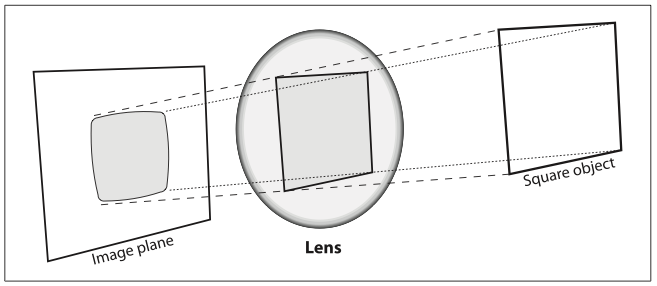
\includegraphics[scale=0.5]{images/radial-disortion.png} 
\caption{Strahlen welche die Linse weiter weg vom Zentrum passieren werden stärker abgelenkt als solche nahe dem Zentrum. Darum erschein die Projektion verzerrt.\protect\cite{learningopencv}}
\label{fig:radial-disortion}
\end{figure}

Tangentiale Verzerrungen werden durch Ungenauigkeiten bei der Zusammensetzung des optischen Systems verursacht. Diese entstehen, wenn die Linse nicht komplett parallel zum Sensor steht.

\begin{figure}[!ht]
\centering
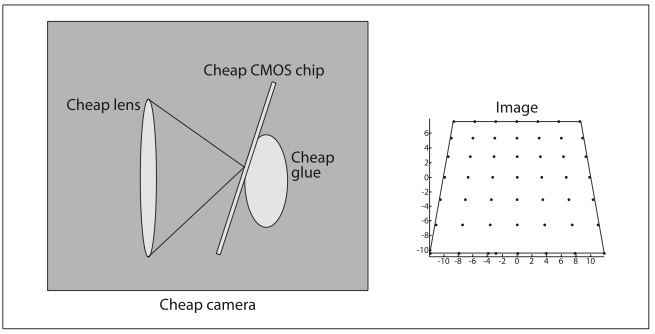
\includegraphics[scale=0.5]{images/tangential-disortion.png} 
\caption{Tangentiale Verzerrung aufgrund von Fehlern im optischen System.\protect\cite{learningopencv}}
\label{fig:tangential-disortion}
\end{figure}

\section{Koordinatensysteme}
Um den Kalibrierungsprozess zu verstehen, muss man auch die einzelnen Koordinatensysteme kennen, welche bei der Aufnahme eines Bildes durchlaufen werden. Deshalb möchten wir diese Hier kurz erläutern.

\paragraph{Weltkoordinatensystem} Dieses ist das Koordinatensystem in welchen die "reale Welt" gemessen wird und ist dreidimensional. Dies ist der Ursprung der Bilddaten.

\paragraph{Standardkoordinatensystem} Dieses dreidimensionale Koordinatensystem hat den Ursprung im Projektionszentrum. Seine Z-Achse verläuft entlang der optischen Achse.

\paragraph{Bildkoordinatensystem} Dieses hat seinen Ursprung beim Schnittpunkt der optischen Achse und der Bildebene. Die x- und y-Achse sind parallel zur X- bzw. Y-Achse des Standardkoordinatensystems.

\paragraph{Pixelkoordinatensystem} Das Pixelkoordinatensystem hat seinen Ursprung beim Korrigierten Punkt $c_x$ \/ $c_y$  und seine x- und y-Achse sind parallel zur x- bzw. y-Achse des Bildkoordinatensystem.

\paragraph{} Während dem Abbildungsprozess durchlaufen die einzelnen Bildimformationen nun diese Systeme wie folgt: Weltkoordinaten $\Rightarrow$ Standardkoordinaten $\Rightarrow$ Bildkoordinaten $\Rightarrow$ Pixelkoordinaten

\section{Implementierung}
Die Funktionalität für die Kalibrierung ist in der Klasse CameraCalibration implementiert. Da alle benötigten Algorithmen bereits in OpenCV implementiert sind, ist der Kalibrierungsprozess relativ einfach umzusetzen. OpenCV selbst verwendet das Verfahren, welches 1998 von Zhang\cite{zhang} entwickelt wurde. Dabei werden die einzelnen Parameter nicht exakt berechnet sondern mittels einer "Maximum likelihood estimation" mit einer hohen Präzision geschätzt. Eine präzise Schätzung erfordert jedoch eine breite Datenbasis. Deshalb reicht es nicht aus, nur eine Aufnahme des Schachbrettmusters als Input zu liefern. Empfohlen werden 15 - 20 Aufnahmen aus möglichst verschiedenen Blickwinkeln. Da die Erkennung des Musters nicht 100\% treffgenau ist, haben wir uns dazu entschieden immer min. 20 Aufnahmen zu verwenden. So können wir davon ausgehen, dass immer mehr als 15 erfolgreiche Erkennungen stattfinden.

\paragraph{}
Die Funktion \textit{CameraCalibration::cornerSubPix} akzeptiert eine Liste von aufnahmen des Schachbrettmusters. Als zweiter Parameter muss die Grösse des Brettes angegeben werden (die Anzahl innerer Eckpunkte in horizontaler und vertikaler Richtung). Dabei sollten die Breite ungerade und die Höhe gerade sein und das Muster sollte breiter als hoch sein. Wir haben uns für ein 6x9 grosses Muster entschieden, da dies die geläufigste Grösse zu sein scheint. Nun wird mittels \textit{CameraCalibration::findChessboardPoints} die Erkennung durchgeführt. Dabei müssen die \textit{objectCorners} (Bildkoordinatensystem) auf einen initialen Erwartungswert gesetzt werden.

\begin{c++code}
for(int i = 0; i < boardSize.height; i++)
{
    for(int j = 0; j < boardSize.width; j++)
    {
		//110 = size of one square on the board
        objectCorners.push_back(
			cv::Point3f(i * 110, j * 110, 0.0f)
		);
    }
}
\end{c++code}

Diese Punkte werden für die Erkennung des Schachbrettes noch nicht benötigt sondern erst bei der Kalibrierung. Anschliessend wird die OpenCV eigene Funktion zur Ermittlung des Musters aufgerufen.

\begin{c++code}
cv::findChessboardCorners(
	image, 
	boardSize, 
	imageCorners, 
	CV_CALIB_CB_ADAPTIVE_THRESH | CV_CALIB_CB_FILTER_QUADS
);
\end{c++code}

Da \textit{cv::findChessboardCorners} nur die ungefähre Position der Eckpunkte ermittelt, müssen die ermittelten Daten mit Hilfe von \textit{cv::cornerSubPix} verfeinert werden. Würde man dies nicht tun, so würde es zu Fehlern bei der Kalibrierung führen. Das genaue Vorgehen der Funktion kann der OpenCV Dokumentation \footnote{\protect\url{http://opencv.willowgarage.com/documentation/cpp/imgproc\_feature\_detection.html\#cv-cornersubpix}} entnommen werden.

\paragraph{}War die Erkennung des Schachbrettes erfolgreich, so entspricht die Anzahl an gefundenen \textit{imageCorners} der zuvor definierten Brettgrösse von 9x6, sprich 54. Alle erfolgreichen Versuche werden anschliessend in einer Liste abgelegt. Was zu beachten ist, und was uns einiges an Zeit gekostet hat, ist, dass die \textit{imageCorners} und die \textit{objectCorners} die gleiche Dimension haben müssen. Ist dies nicht der Fall, so schlägt die Kalibrierung mit einer kryptischen Meldung fehl.

\paragraph{} Nun kann mittels \textit{CameraCalibration::calibrate} die Kalibrierung vorgenommen werden. Diese ist die Voraussetzung für die anschliessende Entzerrung des Bildes welche in \textit{CameraCalibration::remap} stattfindet. Nach jeder Kalibrierung müssen die Daten für die Entzerrung initialisiert werden. Hier ist auch der Punkt, wo wir die Kameramatrix erhalten, welche die intrinsischen Parameter enthält.

\section{Auswertung} Das nun entzerrte Bild kann mit dem Ursprungsbild verglichen werden um zu eruieren ob das optische System Verzerrungen verursacht (Abb. \ref{fig:chessboard-disorted} und \ref{fig:chessboard-undisorted}). Bei den von uns getesteten Kameras konnten wir keine Verzerrungen feststellen. Dabei würden zwei Smartphone-Kameras (iPhone 4 und HTC Desire Z) und zwei Webcams (iSight Kamera eines MacBook Pro und die integrierte Kamera eines HP Notebooks) getestet. Hier stellt sich aber die Frage, ob die getesteten optischen Systeme so kompakt sind, dass die Verzerrungen optisch nicht erfasst werden können oder ob auf Hardwareebene bereits eine Korrektur stattfindet und die API nur Zugriff auf dieses Bild hat. Hierzu konnten wir Seitens der Hardwarehersteller keine Informationen finden.

\begin{figure}[!ht]
\centering
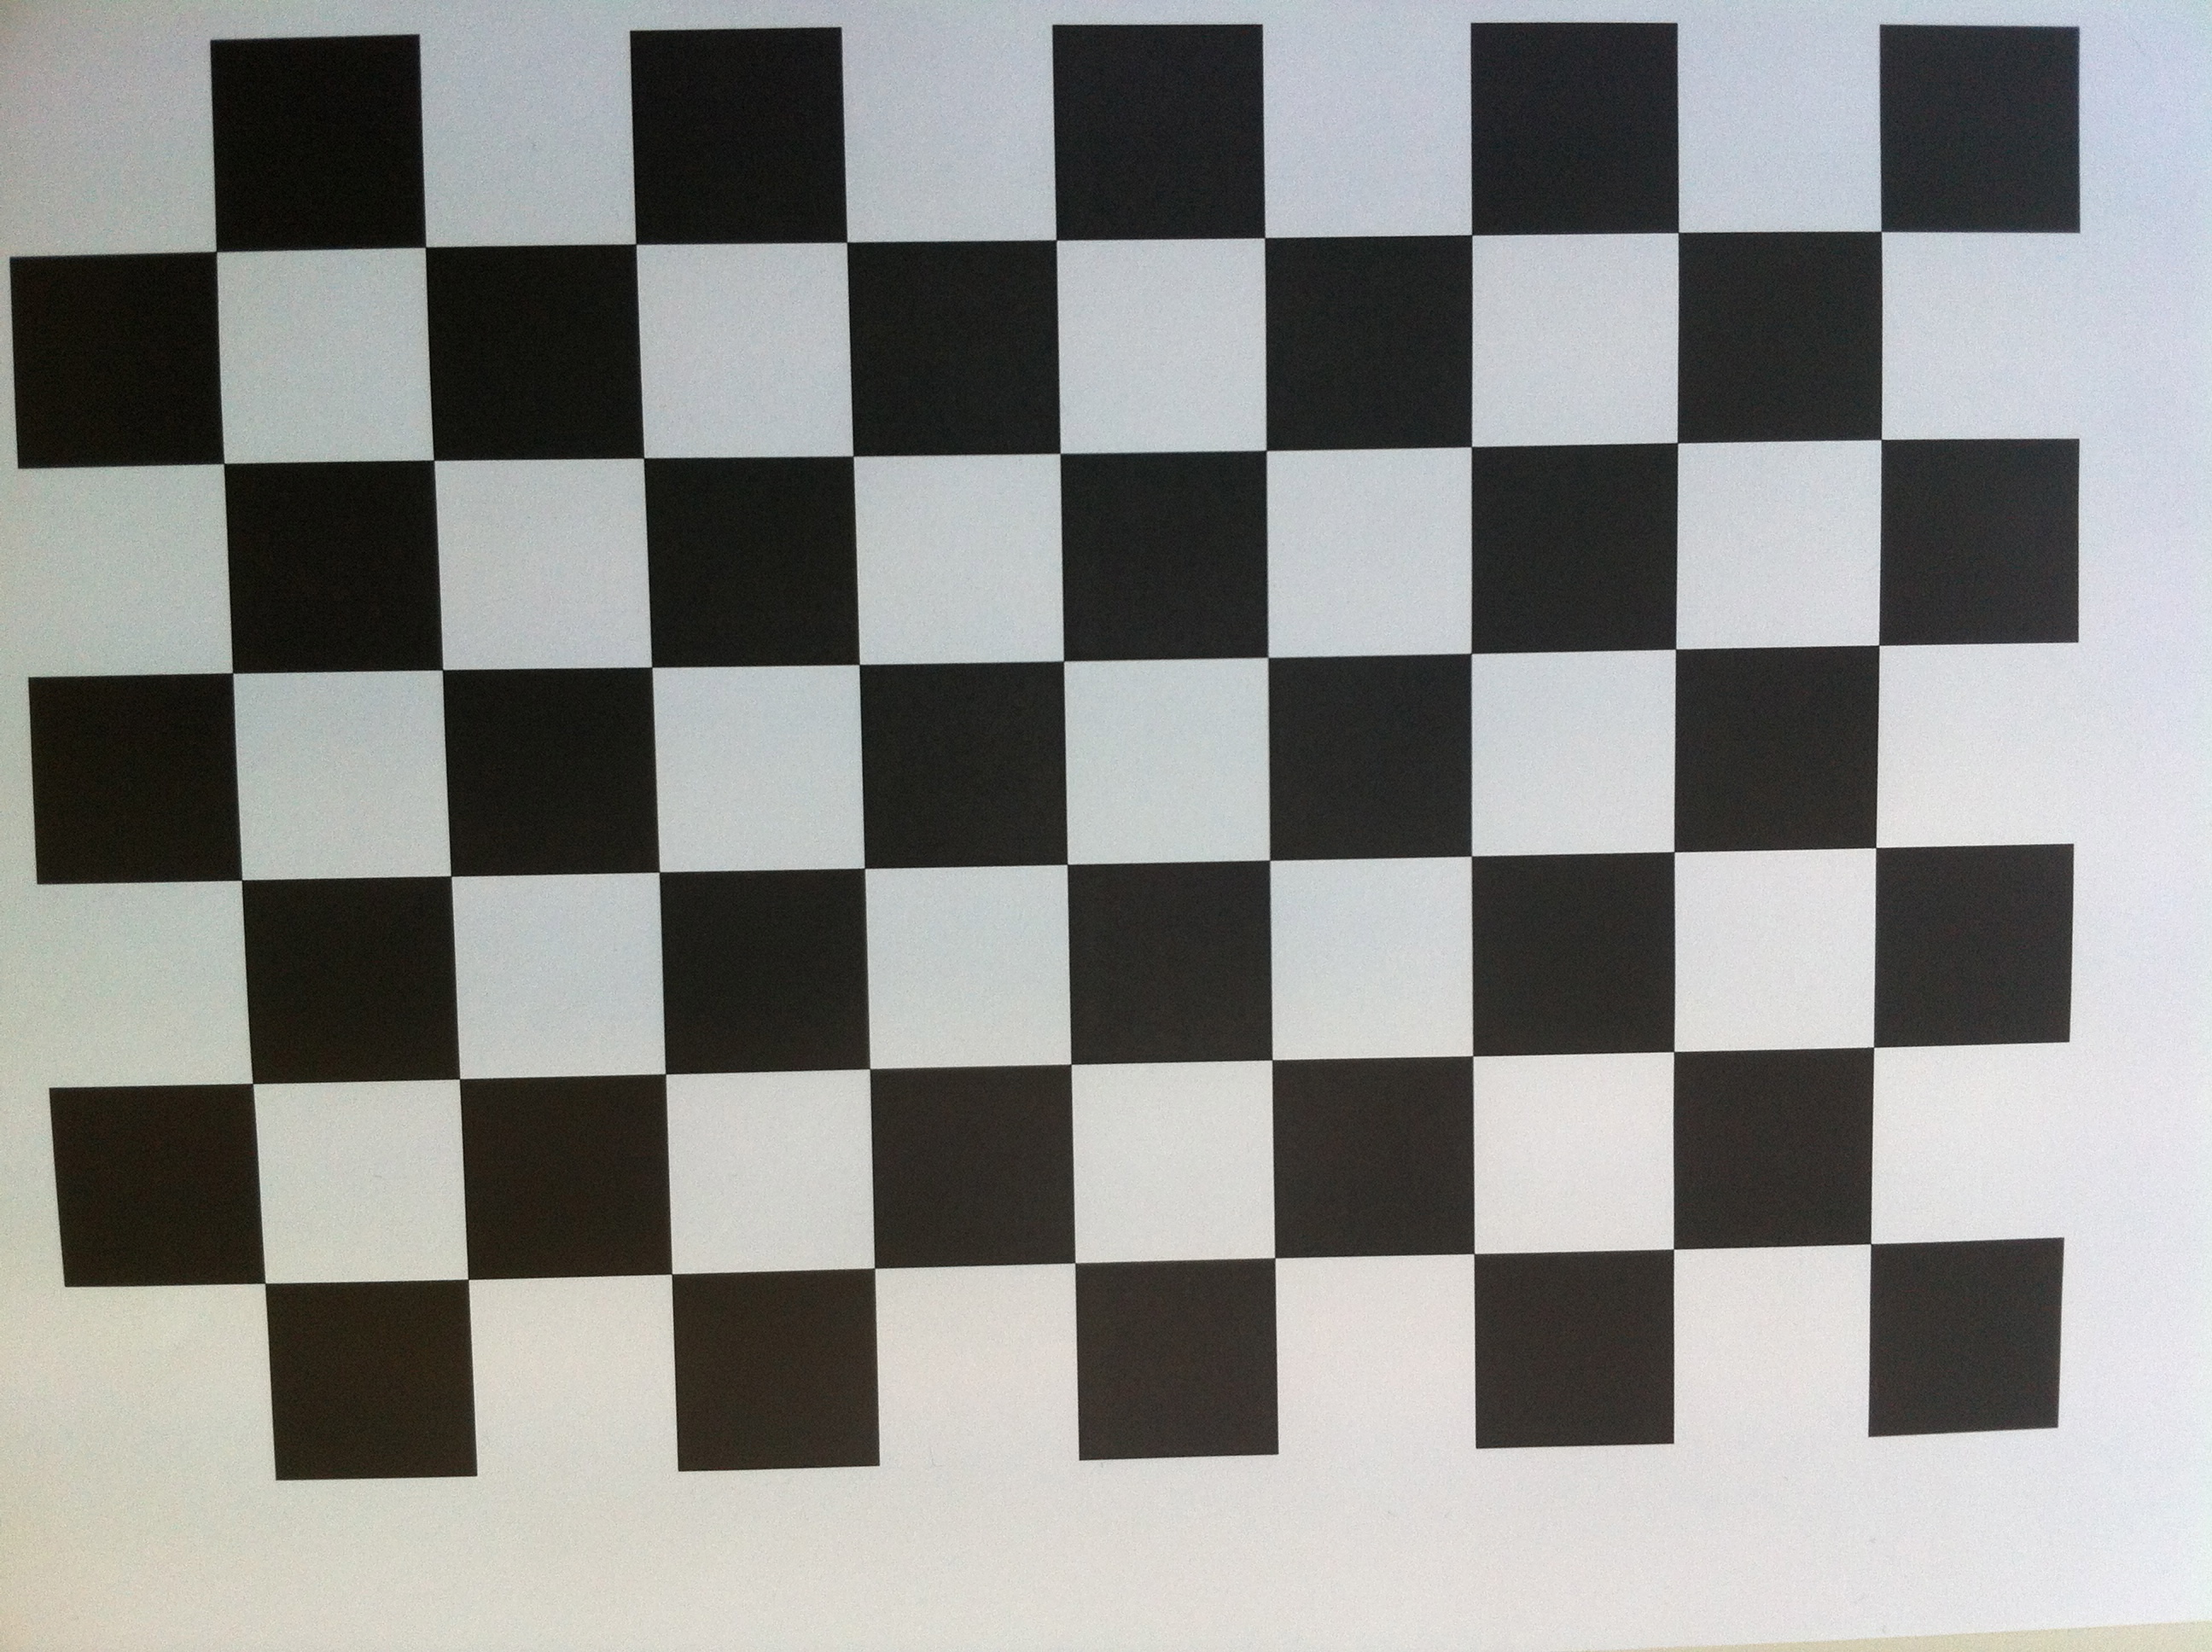
\includegraphics[scale=0.1]{images/chessboard-disorted.jpg} 
\caption{Originalbild}
\label{fig:chessboard-disorted}
\end{figure}

\begin{figure}[!ht]
\centering
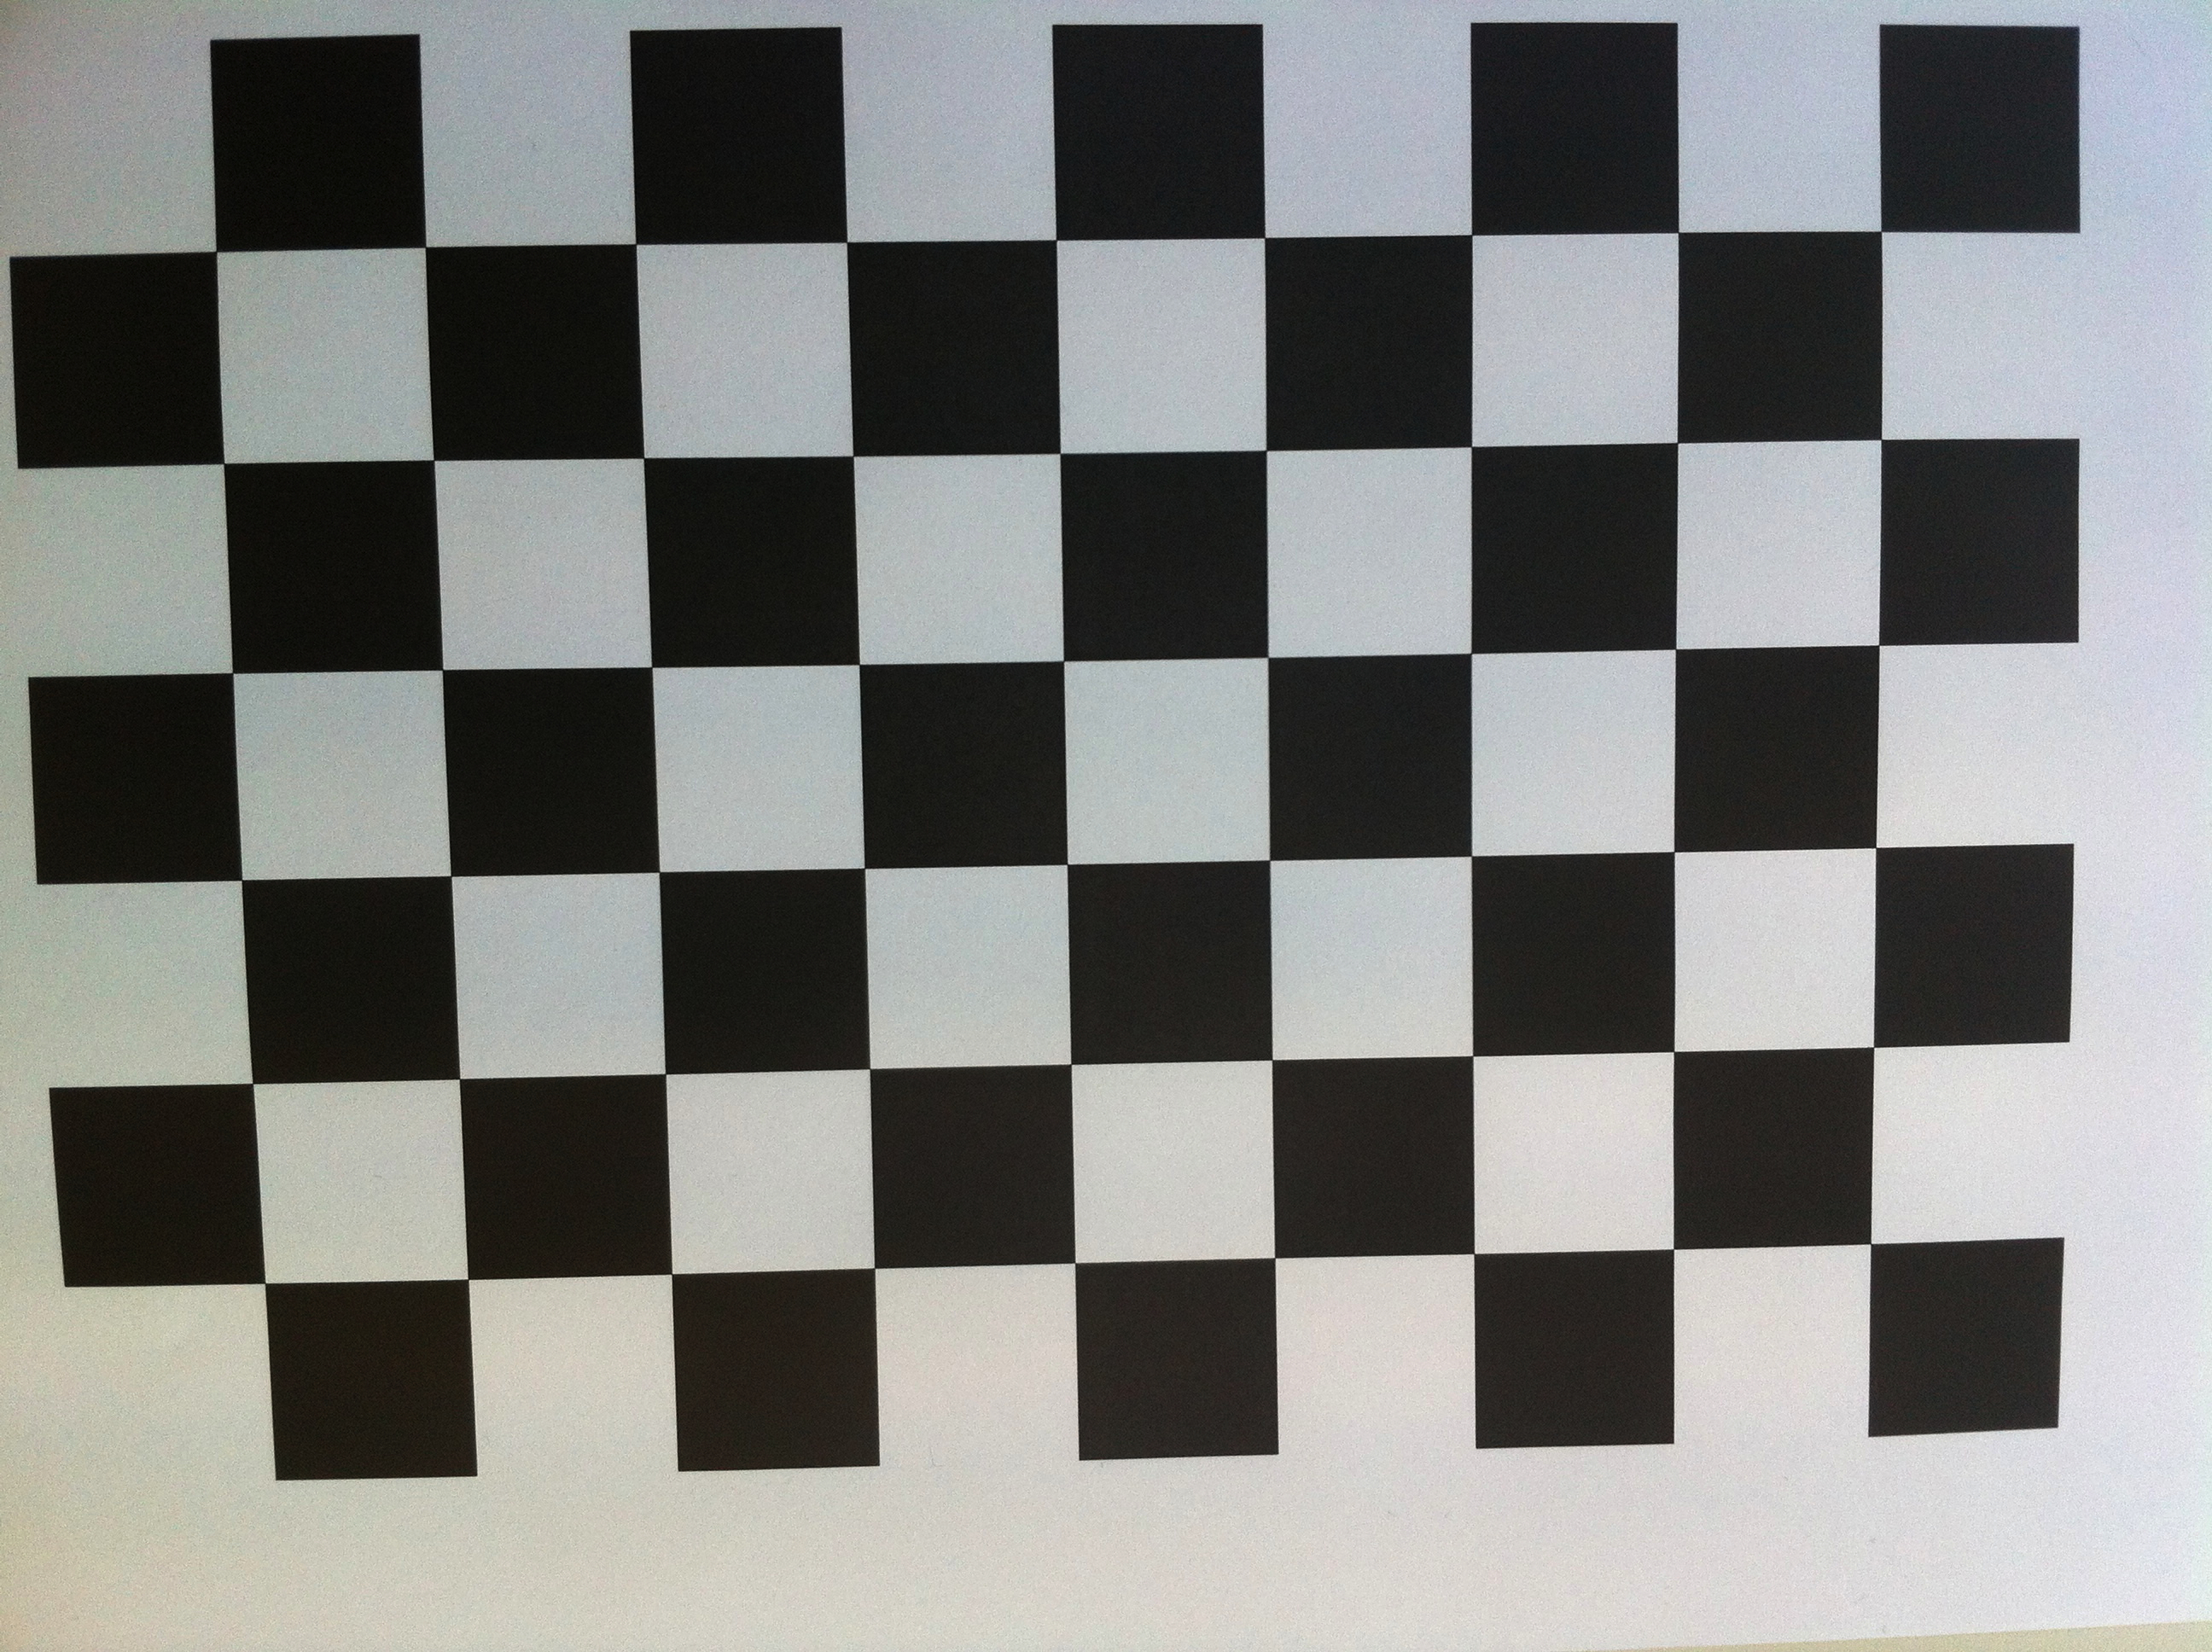
\includegraphics[scale=0.1]{images/chessboard-undisorted.jpg} 
\caption{Entzertes Bild}
\label{fig:chessboard-undisorted}
\end{figure}

\subsection{Perspektive}

\section{Projektionsmodell}
Alle Funktionen in OpenCV arbeiten nach dem sogenannten Pinhole Camera Modell. Dabei werden die 3D-Punkte einer Szene mittels perspektivischer Transformation auf die Bildebene projiziert.

\begin{equation}
\vec{p^p} = K [R|t] \vec{p^i}
\end{equation}

Die ausgeschriebene Form zum besseren Verständnis:

\begin{equation}
\begin{bmatrix}	
p^c_x \\ p^c_y \\ 1
\end{bmatrix} 
=
\begin{bmatrix}
f_x & 0 & c_x \\
0 & f_y & c_y \\
0 & 0 & 1
\end{bmatrix} 
\begin{bmatrix}
r_{11} & r_{12} & r_{13} & t_1 \\
r_{21} & r_{22} & r_{23} & t_2 \\
r_{31} & r_{32} & r_{33} & t_3
\end{bmatrix} 
\begin{bmatrix}
p^i_x \\ p^i_y \\ p^i_z \\ 1
\end{bmatrix} 
\end{equation}

Ein Punkt $(p^i_x, p^i_y, p^i_z)$ im dreidimensionalen Raum wird dadurch auf einen zweidimensionalen Punkt in der Bildebene projiziert. Die Kamera-Matrix $K$ enthält dabei die intrinsischen Parameter und welche nur einmal zu Begin berechnet werden müssen. Die kombinierte Rotations- und Translationsmatrix $[R|t]$ überführt Objekt- in Kamera-Koordinaten, also in die Position, aus der das Objekt von der Kamera gesehen wird. Diese Matrix stellt die extrinsischen Parameter dar und muss anhand einer \textit{Pose Estimation} berechnet werden.

\section{Pose Estimation}
Bei der 3D Pose Estimation wird die Position sowie die Rotation eines Objekts in einem zweidimensionalen Bildes berechnet. Dadurch erhält man die Position des 3D-Objekts im dreidimensionalen Objektraum. Es gibt eine vielzahl an Algorithmen die sich diesem Problem widmen.

\paragraph{}
In OpenCV existieren diverse Funktionen, die gängige Algorithmen zur Positionsbestimmung implementieren. In ARDoor verwenden wir momentan hauptsächlich die Funktion $cv::solvePnP(...)$. PnP wird in der Literatur als \textit{Perspective-n-Point-Problem} bezeichnet, wobei n für die Anzahl an Punktent steht. Bei diesem Problem werden für das im Bild zu suchende Objekt 3D-Punkte definiert, sogenannte \textit{Object Points} oder auch \textit{Feature Points}. Diese Punkte werden mit Bildpunkten (\textit{Image Points}) assoziert, welche bereits vor dem Solve ermittelt werden müssen. Für ARDoor wird der Einfachheit halber das Kalibrations-Schachtbrett als Muster verwendet, da in OpenCV bereits Funktionen existieren, um die \textit{Image Points} des Schachbretts zu ermitteln. Anhand dieser Punktzuordnungen werden mit einem PnP-Algorithmus anschliessend Positions- und Rotations-Vektoren ermittelt.

\paragraph{}
Die $solvePnP$ Funktion in OpenCV unterstützt drei verschiedene Methoden zur Lösung eines PnP Problems:

\begin{itemize}

\item \textbf{Iterative Methode}
Diese Methode basiert auf der Levenberg-Marquardt Optimierung.

\item \textbf{P3P}
Basiert auf der Publikation von X.S. Gao, X.-R. Hou, J. Tang, H.-F. Chang ``Complete Solution Classification for the Perspective-Three-Point Problem''. Es werden exakt vier Objekt- und Bildpunkte benötigt.

\item \textbf{EPnP}
Diese Methode wurde durch F.Moreno-Noguer, V.Lepetit und P.Fua in der Publikation ``EPnP: Efficient Perspective-n-Point Camera Pose Estimation'' entwickelt.

\end{itemize}

\section{Rotation}
Eine 3x3 Matrix ist die geläufigste Methode wenn es darum geht eine Rotation im Raum zu vollziehen. Multipliziert man den Vektor mit der Matrix welche die entsprechenden Parameter enthält, so erhält man als Resultat den rotierten Vektor. Der Nachteil dabei ist, dass man für die Rotation jeder Achse andere Parameter der Matrix anpassen muss. Man kann die drei Matrizen zu einer zusammenfassen, jedoch wird die Prozedur dadurch noch unübersichtlicher. Da die Rotationsmatrizen nur drei Freiheitsgrade haben, ist der Gedanke nahe, die Informationen in einen Vektor abzubilden. Und genau hier setzt die in OpenCV implementierte Rodrigues-Transformation an. Nicht nur für uns Menschen ist ein Vektor einfacher lesbar, auch für numerische Optimierungen ist es einfacher mit einem Drei-Komponenten-Vektor zu arbeiten als mit einer 3x3 Matrix.

\paragraph{}
Rodrigues nutzt die Richtung des Vektors um die Rotationsachse und die Länge des Vektors um den Winkel der Rotation – im Gegenuhrzeigersinn – abzubilden. Sei $r$ ein dreidimensionaler Vektor 

\begin{equation}
\begin{pmatrix} r_x \\ r_y \\ r_z \end{pmatrix}
\end{equation}

Dieser Vektor bildet implizit den Winkel anhand seiner Länge ab.

\begin{equation}
\theta = \sqrt{{r_x}^2 + {r_y}^2 + {r_z}^2}
\end{equation}

Anhand dieser Repräsentation kann die Rotationsmatrix wie folgt wieder hergestellt werden:

\begin{equation}
R = \cos(\theta) * I + (1 - \cos(\theta)) * r * r^T + \sin(\theta) * 
\begin{bmatrix}
0 & -r_z & r_y \\
r_z & 0 & -r_x \\
r_y & r_x & 0
\end{bmatrix}
\end{equation}

Umgekehrt kann man aus der Rotationsmatrix die Rodrigues-Darstellung wie folgt ableiten:

\begin{equation}
\sin(\theta) * 
\begin{bmatrix}
0 & -r_z & r_y \\
r_z & 0 & -r_x \\
r_y & r_x & 0
\end{bmatrix}
= 
\frac{R - R^T}{2}
\end{equation}

Und genau diese zwei Möglichkeiten sind in \textit{cv::Rodrigues} implementiert. Wird als erster Parameter ein 3D-Vektor und als zweiter eine 3x3 Matrix übergeben so wird der Vektor zu einer Matrix transformiert. Will man die Operation umkehren, so müssen nur die Parameter-Typen in umgekehrter Reihenfolge übergeben werden.

\newpage

\chapter{Plattformunabhängigkeit}

In diesem Abschnitt werden die Details der Implementationen auf den beiden Smartphone-Plattformen iOS und Android, sowie den Aufbau unserer ARDoor Library beschrieben.

\section{Grundarchitektur}
Wir haben die Grundarchitektur unserer Applikation laut Abb. \ref{fig:android-architecture} definiert. Die einzelnen Komponenten werden hier kurz beschrieben.

\paragraph{OpenCV}
ist ein quasi-Standard in der nativen Bildverarbeitung und unterstützt eine Vielzahl an Bearbeitungsfunktionen. OpenCV wird in der ARDoor Library für die Bildverarbeitung verwendet.

\paragraph{OpenGL}
wird für das 3D-Rendering benötigt. In der mobilen Welt ist die Library mittlerweile Standard und wird von Android und iOS unterstützt.

\paragraph{ARDoor C++ Library}
Die ARDoor Library enthält den Hauptteil der Applikation. In ihr wird sämtliche plattformunabhängige Logik sowie Verarbeitung und Rendering implementiert. C++ eignet sich  dafür gut, da sowohl von iOS via Objective-C als auch von Android über JNI auf die Library zugegriffen werden kann.

\paragraph{Plattformspezifischer Client}
Pro Plattform wird ein eigener Client implementiert, der den Kamerazugriff übernimmt. Die erfassten Einzelbilder werden an die ARDoor Library zur verarbeitung weitergereicht. Dieser Client sollte nur als Zwischenschicht dienen und deshalb so schlank wie möglich gehalten werden. 


\begin{figure}[!ht]
\centering
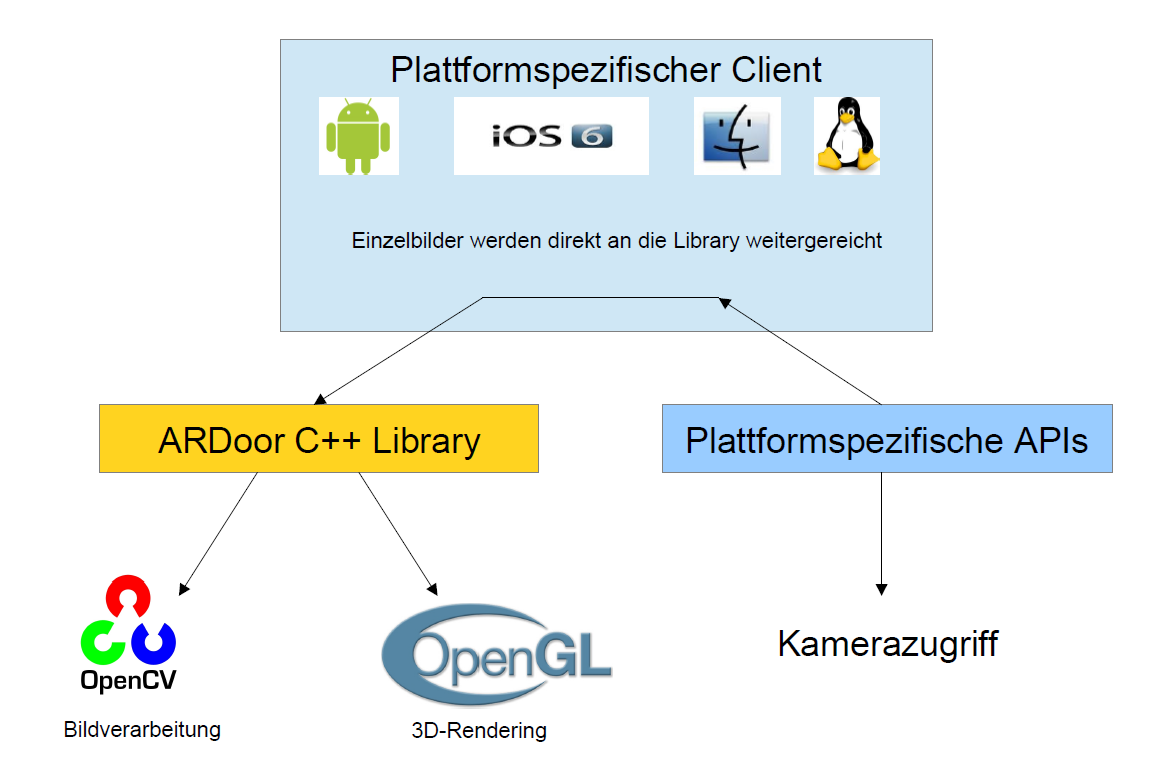
\includegraphics[scale=0.4]{images/architecture.png} 
\caption{Grundarchitektur von ARDoor}
\label{fig:android-architecture}
\end{figure}

\section{Android Plattform}
Zur Entwicklung und zum Testen unter Android wurde ein etwas in die Jahre gekommenes HTC Desire Z verwendet. Es wurde jedoch eine Custom Firmware aufgespielt, welche der Android Version 2.3 entspricht, um bessere Native-Unterstützung zu erhalten. Seit dieser Version, welche dem API Level 9 entspricht, gibt es u.a. die Möglichkeit, eine Native Activity zu implementieren.


\subsection{Native Activity}
Eine Native Activity ist seit Android 2.3 (API Level 9) verfügbar. Eine Native Activity ist im Grunde ein nützlicher Weg, um eine Android App in C/C++ zu implementieren, ohne noch zusätzlichen Wrapper-Code in Java und JNI Code zu schreiben. Mittels der dem Android NDK beiliegenden Library android\_native\_app\_glue kann das Grundgerüst der Native Activity in C/C++ implementiert werden. Dies hat jedoch einige Probleme bereitet.

\paragraph{}
Eines der Probleme war, dass primär zur Entwicklung unter Android Java (via Dalvik VM) als Programmiersprache vorgesehen ist. Ein Grossteil der verfügbaren APIs ist aus diesem Grund nur über Java aufrufbar. Dazu gehört auch die API für den Kamerazugriff. Es wäre zwar möglich aus C++ über JNI mit der Java-API zu kommunizieren, jedoch ist dies aufwändig und fehleranfällig. Auch verursacht JNI einen gewissen Overhead, wodurch ein Aufruf der rein in Java implementierten APIs aus Java-Code heraus schneller ist. JNI Code ist ausserdem sehr mühsam zum lesen und verursacht hohen Wartungsaufwand.

\paragraph{}
Es gibt auch die Möglichkeit mittels der OpenCV Capture-API auf die Kamera des Smartphone zuzugreifen. Das Problem dabei ist, dass OpenCV dazu nicht dokumentierte Funktionen aus einer Android System-Library aufruft. Dies funktioniert leider nicht mit allen Geräten. Da die aufgerufenen Funktionen nicht zu einer offiziellen, stabilen API gehören, können diese bei einer neuen Android-Version ändern und die Entwickler von OpenCV müssten diese Unterstützung zuerst implementieren.

\paragraph{}
Was bei der Native Activity auch beachtet werden muss ist, dass die ganzen Android-Events, z.B. Input oder App-Lifecycle-Events, selber abgeholt und weiterverarbeitet werden müssen. Dadurch schreibt man quasi von Grund auf ein eigenes Applikationsframework auf nativer Basis.


\subsection{JNI Zugriff}
Die andere Möglichkeit ist der Zugriff auf C/C++ via JNI. Die Grund-App wird dabei in Java implementiert. In der nativen Library werden bei dieser Methode spezielle JNI-Funktionen implementiert, die aus Java heraus aufgerufen werden können.

\paragraph{}
Bei dieser Variante haben wir zwar immer noch die Java-Schicht, jedoch kann dadurch auf eine stabile und funktionierende API zurückgegriffen werden. Auch ist es einfacher später ein GUI zu implementieren, z.B. zur Auswahl des zu projizierenden 3D-Models.


\section{iOS Plattform}
Zur Entwicklung der iOS Version der Applikation haben wir ein iPhone 4 eingesetzt welches einen A4 Prozessor basierend auf der ARMv7-A\footnote{\url{http://www.arm.com/products/processors/instruction-set-architectures}} Architektur besitzt. Die plattformspezifischen Funktionen wurde in Objective-C geschrieben. Im Gegensatz zu Android braucht es auf der iOS Plattform keine Bridge um C++ Code ausführen zu können. Da Objective-C wie auch C++ eine Obermenge von C ist, können C++ Klassen in der gewohnten Syntax direkt verwendet werden. Dies ist einer der grössten Vorteile der iOS Plattform. Fast alle bestehenden C und C++ Bibliotheken können ohne Umwege Verwendet werden.

\paragraph{}
Einen weiteren Vorteil welchen Objective-C bietet ist, dass alle Klassen grundsätzlich Beliebig erweitert werden können. So konnten wir z.B. die \textit{UIImage} Klasse um Funktionen erweitern, welche es uns ermöglichen den Inhalt eines \textit{UIImage} in eine \textit{cv::Mat} Struktur umzuwandeln und umgekehrt (zu Finden in der Klasse \textit{UIImage+OpenCV}). Somit gestaltete sich der Datenaustausch zwischen den plattformspezifischen Komponenten und unserer unabhängigen ARDoor Library sehr einfach.

\subsection{Kamerazugriff} Der Kamerazugriff ist eher etwas komplex gestaltet unter iOS. Glücklicherweise ist die Dokumentation von Apple sehr ausführlich und bietet zu allen komplexen Prozessen Codebeispiele. So auch für den Kamerazugriff. Dies hat uns einiges an Zeit gespart, denn ohne diese Beispiele muss man sehr tiefgehende Kenntnisse – ja man muss schon fast ein Experte sein – von iOS haben um den Kamerazugriff zu konfigurieren. Die Komponenten für Audio und Video In- und Output befinden sich im AVFoundation Framework Welches wiederrum CoreMedia und CoreVideo verwendet (Abb. \ref{fig:avfoundation}).

\begin{figure}[!ht]
\centering
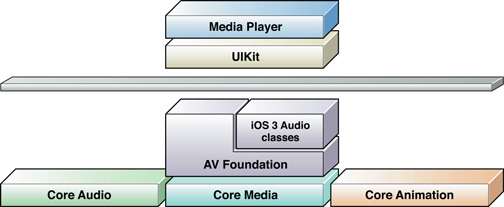
\includegraphics[scale=0.6]{images/avfoundation.jpg} 
\caption{Aufbau des Medienzugriffes unter iOS, Quelle: \protect\url{http://developer.apple.com/library/ios}}
\label{fig:avfoundation}
\end{figure}

Das Setup für den Kamerazugriff gestaltet sich dann wie folgt:

\begin{itemize}
\item Als erstes muss eine Instanz von \textit{AVCaptureDevice} aufgesetzt werden. Diese repräsentiert das Gerät über welches der Input geliefert wird.
\item Über eine \textit{AVCaptureDeviceInput} wird der Datenstrom des Eingabegerätes gesteuert.
\item Mittels \textit{AVCaptureVideoDataOutput} wird die Ausgabe der Daten, in unserem Fall auf ein UIImage, gesteuert.
\item Die letzte Komponente ist die \textit{AVCaptureSession}, welche den Datenstrom von \textit{AVCaptureDeviceInput} zu \textit{AVCaptureVideoDataOutput} steuert.
\end{itemize}

Der Afbau ist in Abb. \ref{fig:ios-capture-overview} visualisiert. Der Code für das Setup befindet sich in \textit{VideoCaptureViewController::createCaptureSessionForCamera}. Obwohl der Kamerazugriff eher komplex aufgebaut ist, bietet er auch einige vorteile. Es ist einfach mehrere Input-Devices wie eine Kamera und ein Mikrofon zusammenzufassen. Weiterhin kann man auch sehr einfach das Input-Device austauschen, z.B. die Backface-Kamera mit der Frontface-Kamera. Beides, ohne dass die darunterliegenden Layer etwas davon mitbekommen.

\begin{figure}[!ht]
\centering
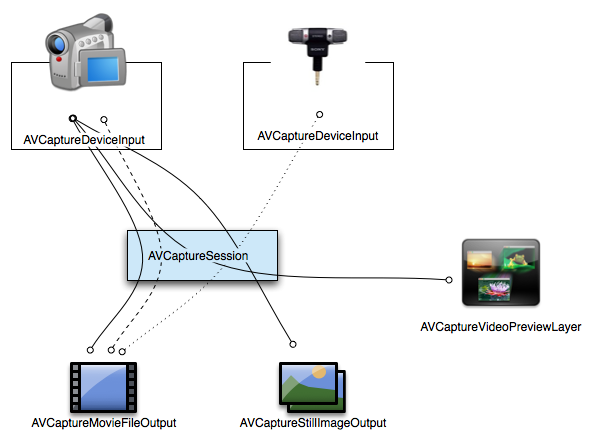
\includegraphics[scale=0.6]{images/ios-capture-overview.png} 
\caption{Aufbau des Medienzugriffes unter iOS, Quelle: \protect\url{http://developer.apple.com/library/ios}}
\label{fig:ios-capture-overview}
\end{figure}

\subsection{OpenCV unter iOS}
OpenCV lässt sich unter iOS mittlerweile sehr einfach einbinden. Noch bis vor kurzem musste man die Bibliothek noch selbst für die ARM-Plattform kompilieren, was sich als sehr mühsam erwies. Jedoch bieten die OpenCV-Macher mittlerweile vorkompilerte Binaries in Form eines Framework-Bundles an. Die Framework-Bundle Form hat den Grossen vorteil, dass die Binaries mit relativen Pfaden gelinkt sind. So ist das Deployment viel einfacher. Andernfalls müsste man nach der Kopilierung die Linker-Pfade mittels otool vor dem Deployment anpassen. Eine iOS App wird zuerst lokal auf dem Entwicklungsrechner Kompilert und danach auf das Endgerät (oder den iOS Simulator) installiert. Da die Verzeichnisstrukturen nicht auf beiden Geräten identisch ist, währen somit die Linker-Pfade nicht korrekt wenn sie absolut wären.

\paragraph{Performance} Die Performance von OpenCV unter iOS ist nicht optimal. Innerhalb von OpenCV wird standardmässig OpenMP für die Parallelisierung eingesetzt. Da jedoch OpenMP bisher noch nicht auf ARM portiert wurde, wird die Leistung des Prozessors nicht voll ausgeschöpft. So drückt eine Sobel-Live-Kantendetektion des Kamerabildes die Framerate bereits auf ca. 13 fps runter. Die Erkennung einen Schachbrettmusters mittels \textit{cv::findChessboardCorners} bringt es nicht einmal mehr auf ein fps. Eine Möglichkeit hier die Performance zu Optimieren währe Grand Central Dispatch (GCD) einzusetzen. Dies ist die Objective-C spezifische Multithreading Umgebung von Apple. Seit der Version 2.4.3\footnote{\url{http://code.opencv.org/projects/opencv/wiki/ChangeLog}} besitzt OpenCV eine \textit{parallel\_for} Implementierung für diverse Multithreading Backends, unter anderem auch für GCD. Eine weitere Möglichkeit die Leistung der Anwendung zu optimieren währe, wo möglich, Operationen mittels NEON\footnote{\url{http://www.arm.com/products/processors/technologies/neon.php}} umzusetzen. NEON ist ein SMID Instruction Set, ähnlich wie MMX von Intel, welches parallele Operationen auf einer Instruktion erlaubt. Beide Optionen gilt es während der Bachelor-Thesis zu erforschen.

\section{Desktop Platform}
Da die Performance von OpenCV auf den mobilen Geräten suboptimal ist und es auf Grund der tiefen Frameraten sehr mühsam wurde die Applikation zu testen, haben wir uns dazu entschieden auch eine Desktop-Variante umzusetzen. Als Grundlage dafür haben wir das QT-Framework eingesetzt. Zu begin haben wir auch noch eine Mac OS X spezifische App entwickelt. Jedoch wurde der Aufwand zwei Desktop Varianten zu entwickeln schlicht zu hoch, da wir uns in beide Plattformen zuerst tiefer einarbeiten hätten müssen. Deshalb haben wir uns dazu entschlossen, nur noch die QT-Variante weiterzuentwickeln. Mittels QT-Framework kann sowohl unter Mac OS X als auch unter Linux entwickelt werden, welche die Zielplattformen für die Desktop App waren. Einzig bei der Einbindung von Libraries wie OpenCV und bei der Einbindung von einigen Header-Dateien müssen Weichen für OS X und Linux eingebaut werden, da die Namensgebung nicht immer identisch ist. 
\paragraph{}
Eine wichtige Einstellung welche vorgenommen werden musste ist die Deaktivierung des QML-Debuggers. Solange diese Option aktiv war, wurde der eigentliche C++ Debugger nicht korrekt ausgeführt. Das führte dazu, dass Fehler im Code nicht erkannt werden konnten. Die Applikation verhielt sich nicht wie erwartet, gleichzeitig wurden beim Kompilieren aber keine Fehler ausgegeben; Breakpoint wurden einfach ignoriert. Weiterhin verhielt sich das Event-Handling innerhalb von QT nicht wie spezifiziert, solange der QML-Debugger aktiv war. Diese Situation führte zu einer erheblichen Verzögerung in der Entwicklung, bis dieser Konfigurationsparameter als Ursache lokalisiert wurde. Der Grund für dieses Fehlverhalten könnte sein, das wir nicht QML für die Erstellung des UI einsetzen, sondern das XML basierte System. Wahrscheinlich gibt es Inkompatibilitäten zwischen den zwei Libraries.
\paragraph{}
Ein weiteres Hindernis welches wir hatten war die Kompilierung von OpenCV unter Mac OS X. Leider bieten die Hersteller keine precompiled Binaries für Mac OS X an. Das Problem bestand darin, dass der Linker falsche relative Pfade zu OpenCV gesetzt hat. Erst als wir einen Patch für OpenCV\footnote{\url{http://code.opencv.org/issues/2037}} entdeckt hatten, welcher es erlaubte die Bibliothek als Framework zu verpacken, konnte OpenCV problemlos unter Mac OS X betrieben werden. Ein Problem welches bis heute noch ungelöst ist, ist die OpenGL-Unterstützung innerhalb von OpenCV unter Mac OS X. Obwohl der nötige Kompilierungsparameter \textit{WITH\_OPENGL} korrekt gesetzt wurde, wurde OpenCV ohne OpenGL-Unterstützung kompiliert. Dies führte dazu, dass wir viele Beispielapplikationen nicht Ausprobieren, da diese OpenGL-basierte GUIs verwenden.

\section{Calibration Dialog}
Der Calibration Dialog dient dazu, die Kameraparameter zu ermitteln. Dies muss grundsätzlich nur einmal zu Begin gemacht werden. Die gewonnenen Daten werden anschliessend in eine Konfigurationsdatei abgelegt. Die Datei wird im systemspezifischen Konfigurationsverzeichnis abgelegt.

\section{Mainwindow}
Das Mainwindow ist der Hauptteil der Applikation. Innerhalb von diesem wird die Augmented Reality Szene dargestellt.

\section{ARDoor Library}
Wir haben uns zum Ziel gesetzt, die ARDoor Library möglichst modular aufzubauen, so dass wir verschiedene Komponenten einfach austauschen könnten und wir somit flexibel in der Entwicklung sind. Da wir bei der Entwicklung sehr viele Dinge ausprobiert haben und ständig Sachen neu implementiert haben, konnten wir dies nicht zu 100\% umsetzen. Sobald wir eine erste funktionierende Version mit Positionsbestimmung und korrektem Rendering haben, werden wir ein generelles Code-Refactoring durchführen.

\section{ImagePipeline}
Eine der Hauptkomponente der ARDoor Library ist die Image Pipeline. Der Grundgedanke dahinter ist, dass die verschiedenen Schritte zur Bildbearbeitung und -verarbeitung in sich geschlossenen modularen Klassen - einem \textit{ImageProcessor} - implementiert werden. Wir erhoffen uns davon eine einfachere Entwicklung, da wir dadurch die verschiedenen Verarbeitungsschritte einfach austauschen oder in der Reihenfolge der Ausführung neu positionieren können.

\paragraph{}
Ein weiterer Grundgedanke für diesen Aufbau war, dass wir so einfach Debugmöglichkeiten einbauen könnten: Man könnte einen einfachen Debug ImageProcessor, der das aktuelle Bild nur darstellt und nicht verändert, implementieren und diesen an eine beliebige Position der Pipline setzen.

\paragraph{}
Implementiert haben wir die Pipeline so, dass für jedes Bild, welches wir von der Kamera erhalten, eine OpenCV-Matrix cv::Mat erzeugt wird. Diese wird der Pipeline nun zur Verarbeitung übergeben. Die Pipeline übergibt diese Matrix dem aktuellen ImageProcessor, der eine weitere Matrix als Rückgabewert liefert. Die zurückgegebene Matrix wird jeweils als Eingabe für den nächsten ImageProcessor in der Pipeline verwendet. Zum Schluss wird von der Pipeline das finale Bild nach allen Verarbeitungsschritten zurückgegeben. Dieser Ablauf ist in Abbildung \ref{fig:image-pipeline} grafisch dargestellt.

\begin{figure}[!ht]
\centering
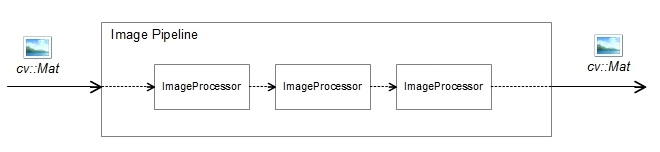
\includegraphics[scale=0.8]{images/image-pipeline.jpg} 
\caption{Aufbau der Image Pipeline}
\label{fig:image-pipeline}
\end{figure}

\section{RenderingContext}
Eine weitere Komponente der Library ist der RenderingContext. Die primäre Aufgabe dieser Komponente ist das Rendering der 3D-Modelle einer Szene sowie das korrekte setzen der Projektions- und ModelView-Matrizen. Diese strikte Trennung ist im Moment noch nicht konsequent umgesetzt, da der RenderingContext auch Aufgaben der Pose Estimation übernimmt.  

\newpage

\chapter{Fazit}

Insgesamt sind wir mit unserer Arbeit zufrieden und konnten unser Hauptziel zum gr�ssten Teil erreichen. Wir k�nnen T�ren in einem Livebild erkennen und deren Position und Rotation bestimmen. Die Arbeit war f�r uns eine grosse Herausforderung, da wir beide vorher nur wenig bis gar keine Erfahrung auf den unterschiedlichen Gebieten dieses Projekts hatten.

Probleme gibt es noch bei Erkennung von seitlich betrachteten T�ren. Hier funktioniert die Erkennung noch nicht zuverl�ssig. Wir haben zu sp�t realisiert, dass wir f�r die perspektivische Erkennung zus�tzliche Verfahren h�tten evaluieren sollen, z.B. die Klassifizierung von Linien anhand der Tendenz zu einem Fluchtpunkt.

% TODO evtl. mit Resultat verschmelze?


Da wir haben mit unserer Arbeit in erster Linie eine Grundlage geschaffen haben, gibt es definitiv zus�tzliches Optimiers- und Erweiterungspotential.

Sinnvoll w�re eine Optimierung der Performance der Algorithmen, besonders im Bereich der T�rerkennung. Hier haben wir prim�r auf die Funktionalit�t konzentriert. 

Ein wichtiger n�chster Schritt wird sein, die Anwendung auf mobile Plattformen zu portieren. Durch die immer h�ufigere Verbreitung von Smartphones und die M�glichkeit, Informationen an Ort und Stelle abzurufen, oder im Falle von Augmented Reality direkt einzublenden, sind solche Ger�te eine gew�nschte Zielgruppe. 

Ein Ausblick in die Zukunft der Augmented Reality sieht ebenfalls vielversprechend aus. Grosses Aufsehen sorgte diesbez�glich vorallem Google, die mit ihrem Produkt Glass versuchen Augmented Reality Massentauglich zu machen. Besonders in Alltagssituation k�nnte Augmented Reality eine grosse Rolle einnehmen, beispielsweise durch Navigationshilfen in Autos, die n�tzliche Informationen direkt auf die Frontscheibe projizieren.

Aber auch f�r unseren Spezialfall der Augmented Reality kann man sich verschiedene Anwendungszwecke vorstellen. Das Einkaufen k�nnte interaktiver werden, indem Dinge wie M�bel als Modelle auf das eigene Smartphone geladen werden. Mittels einer Augmented Reality App k�nnen diese direkt in der aktuellen Umgebung von allen Seiten betrachtet werden. Dies k�nne zudem mit aufkommenden Techniken wie NFC (Near Field Communication) erweitert werden: Man stelle sich eine Einkaufstour durch ein M�belhaus seiner Wahl vor. Mittels NFC k�nnen 3D-Modelle von M�beln direkt auf das Smartphone geladen werden. Sp�ter kann man die ausgesuchten Gegenst�nde in der eigenen Wohnung virtuell platzieren und dadurch eine bessere Kaufentscheidung f�llen.


\newpage

\chapter{Ausblick}

In der nun bevorstehenden Bachelor-Thesis geht es nun als erstes darum, den Fehler in der perspektivischen Projektion zu beheben. Dies ist der Grundstein für die weitere Arbeit. In einem weiteren Schritt muss das Marker-basierte Konzept abgelöst werden. Wollen wir Türen automatisch erkennen, so müssen wir ohne jegliche Marker auskommen. Diese zwei Punkte sollen vorerst ebenfalls in der Desktop App umgesetzt werden.
\paragraph{}
Basierend auf einer funktionierenden Desktop Anwendung, können dann die mobilen Applikationen entwickelt werden. Der Hauptteil der Arbeit wird hier darin bestehen, Optimierungsmöglichkeiten zu finden um die Framerate zu erhöhen. Mögliche Mittel sind hier OpenCL aber auch NEON. NEON ist zwar eine ARM-Spezifische Technologie, da aber sowohl alle gängigen Android Devices als auch alle iPhone ab der vierten Generation auf ARMv7 und höher aufbauen, ist NEON auch in einem gewissen Mass plattformunabhängig.
\paragraph{}
Da wir gegen Schluss unseres Projekts hauptsächlich auf dem Desktop entwickelt haben und wir möglichst schnell etwas visuell darstellen wollten, haben wir die grafische Darstellung vor allem mit alten OpenGL-Funktionen umgsetzt. Die moderne Art der OpenGL-Programmierung basiert vor allem auf direkter Programmierung der GPU via Shader und verwendet das \textit{OpenGL Core Profile}. Da auf Smartphones OpenGL ES 2 verwendet wird, wollen wir während der Bachelor-Thesis ebenfalls unsere Codebasis auf diese Version migrieren, so dass wir auf sämtlichen Plattformen denselben OpenGL-Code wiederverwenden können.
\paragraph{}
Als letztes Ziel haben wir eine Saubere und gut dokumentierte Codebasis gesetzt. Auch wenn wir unsere Ziele eventuell nicht zu 100\% erreichen, soll die Arbeit als Grundlage für weitere Forschungen verwendet werden können. Hierzu muss die Hürde für die Übernahme unserer Arbeit so tief wie möglich gehalten werden.

\newpage


\newpage
\begin{thebibliography}{5}

\bibitem {learningopencv}
Bradski, Gary / Kaehler Adrian:
Learning OpenCV: Computer Vision with the OpenCV Library.
Sebastopol: O'Reilly Media, Inc.

\bibitem {zhang}
Zhang, Zhengyou (1998): A Flexible New Technique for Camera Calibration. 
Redmond: Microsoft Research.

\bibitem {escalera}
de la Escalera, Arturo / María Armingol, Jose: Automatic Chessboard Detection for Intrinsic and Extrinsic Camera Parameter Calibration. 
Madrid: Universidad Carlos III de Madrid.

\end{thebibliography}
\end{document}
